\chapter{Architecture}
% TODO make diagrams more readable, discussion?

  The framework has been implemented as a 3-tier architecture. This allowed us to easily
  separate responsibilities and minimise coupling. The architecture focuses on allowing
  third party integrations easily with the use of the interceptor architectural pattern.
  To make it easy for clients to use the framework, a server is supplied which exposes
  a REST API. A pluggable adapter is used in order to allow the integration of other
  database systems which is an important feature.

  \section{Architectural Diagram}
  TODO

  \section{Package Diagram}
    \begin{figure}[H]
        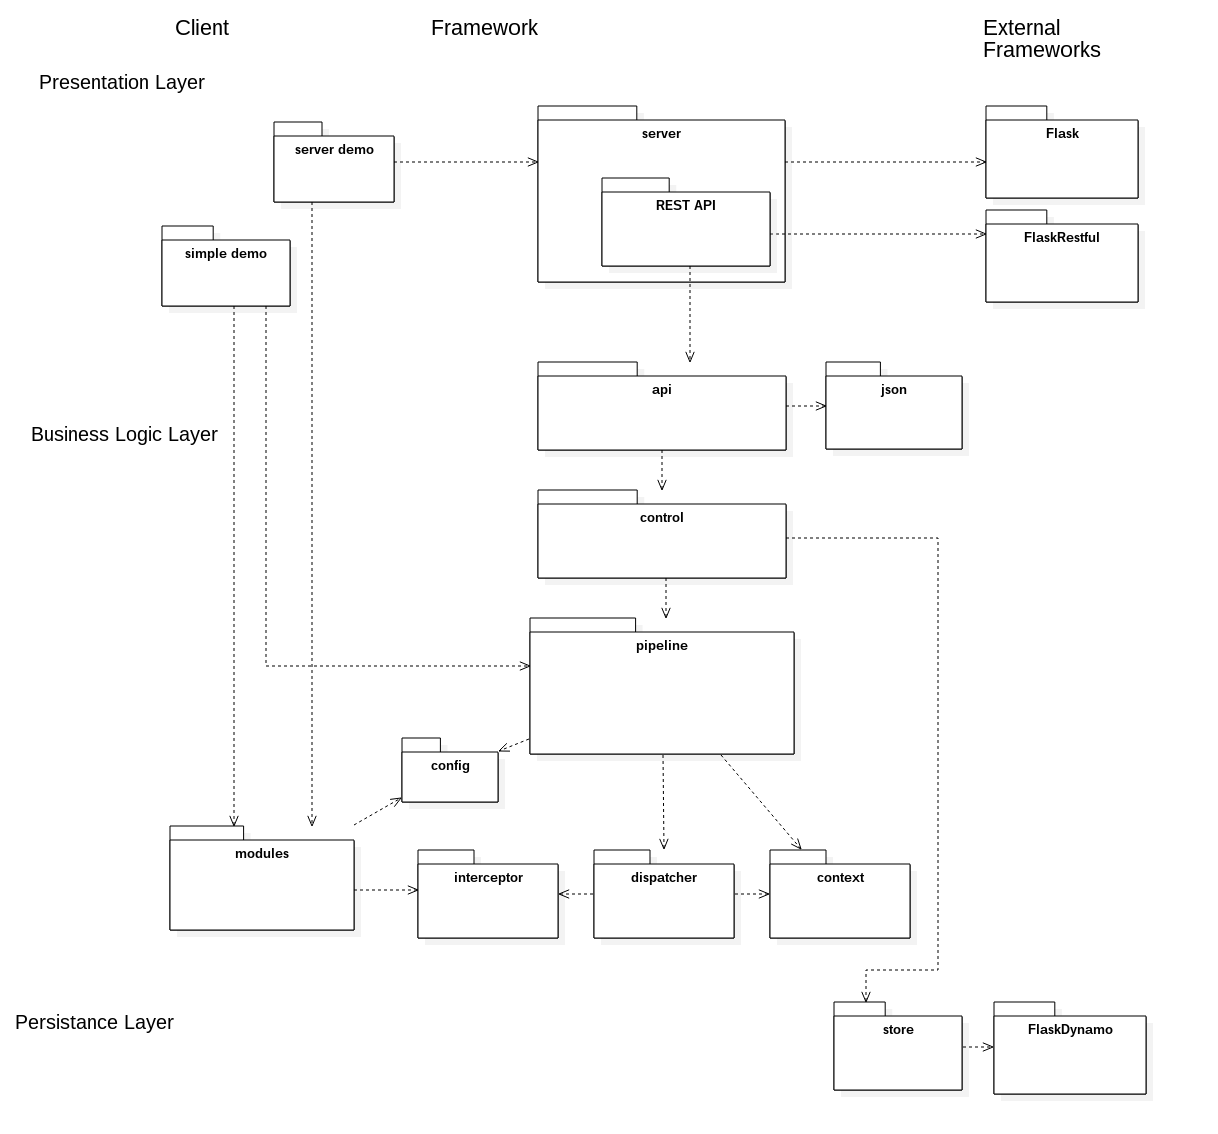
\includegraphics[width = 1.2\linewidth]{diagrams/architecture.png}
        \caption{High Level Architecture}
        \label{fig:high_level_architecture}
      \end{figure}

  \section{Class Diagram}
    \begin{figure}[H]
        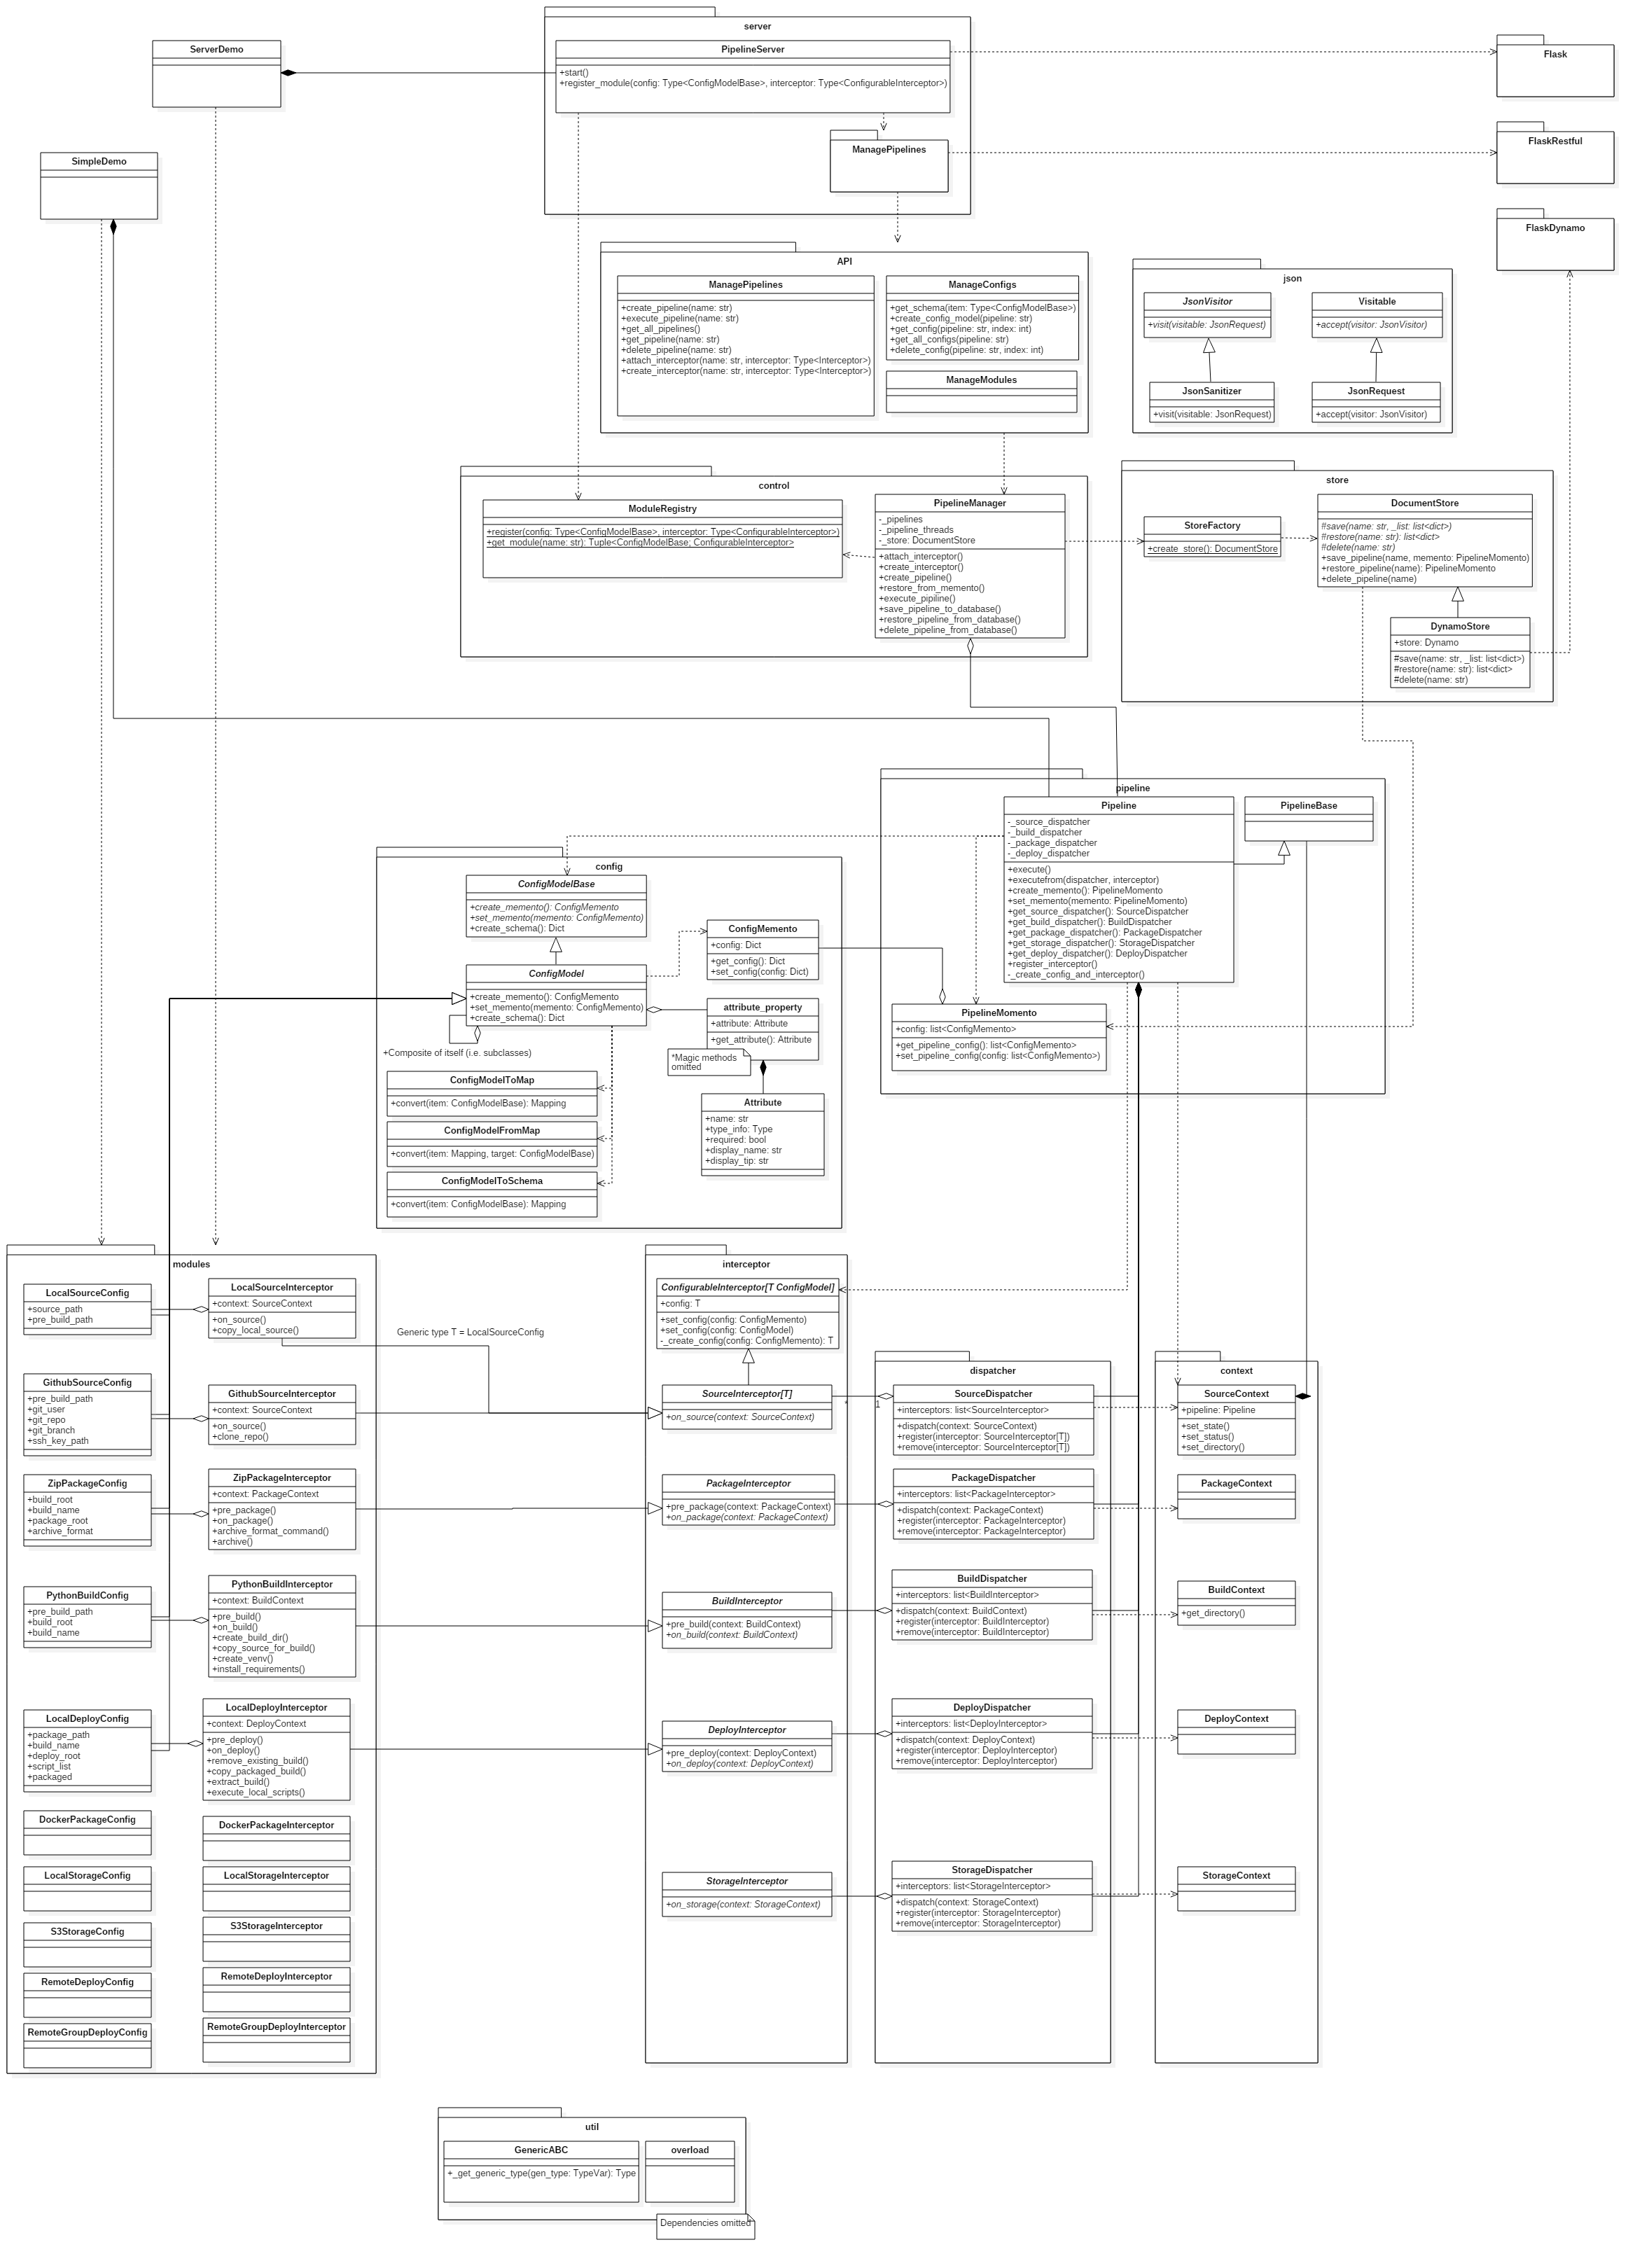
\includegraphics[width = 1.2\linewidth]{diagrams/architecture_classes.png}
        \caption{Architecture Class Diagram}
        \label{fig:architecture_classes}
      \end{figure}

    \section{Class Diagram Fragments}
    TODO
    
   
   \section{Sequence Diagram}
	   \begin{figure}[H]
	   	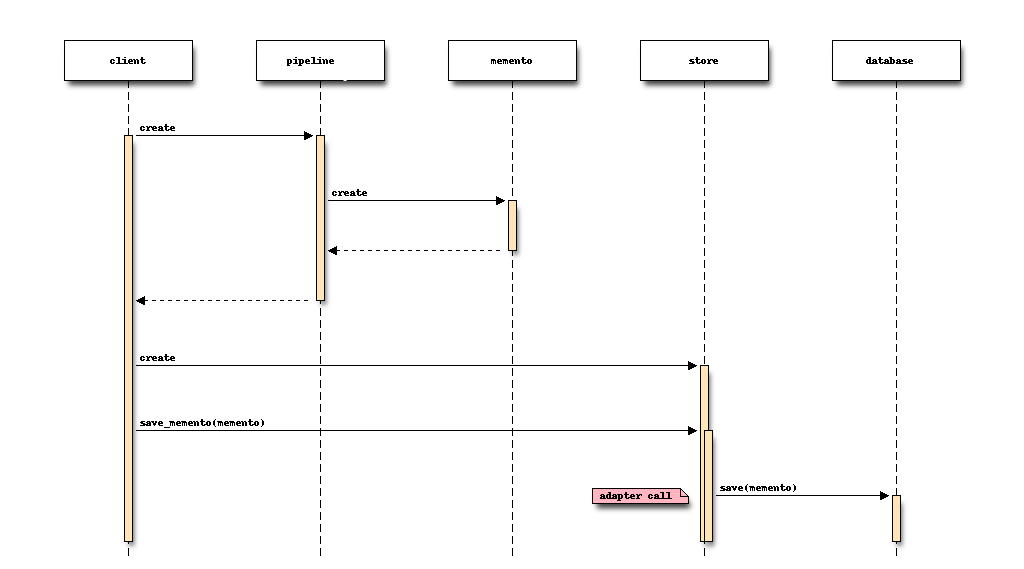
\includegraphics[width = 1.2\linewidth]{diagrams/sequence_diagram.png}
	   	\caption{Pluggable Adapter Sequence Diagram}
	   \end{figure}

TODO structural diagram
